\subsection{Introduction}
In the distributed systems the natural distribution of the system complicates the synchronization, since we don't have a single local clock and/or a globally shared memory. For this reason there are some algorithms and protocols which aim to solve these problem, such as the synchronization between two or more machine clocks and the order of events in a distributed system.

\subsection{Physical clocks synchronization}
When we want to synchronize two or more physical clocks we have, basically, to face up with two requirements: \textbf{accuracy} and \textbf{agreement}. For \textit{accuracy} we mean that all clocks must be synchronized against a single one, with accurate time information, while, by the term \textit{agreement} we mean that all hosts must synchronize their clocks in the same way and with the same references between them.

When synchronizing clocks, one important thing is that temporal \textbf{monotony} must be preserved. In fact, if I discover to be ahead of time, typically I delay my timer, because it's dangerous go back with the timer because I can cause crashes.

\subsubsection{GPS}
One possible way to synchronize clocks is based on \textit{GPS (Global Position System)} mechanism. In other words, the idea is to exploit the \textit{GPS} procedure used to calculate the position of an object and, since the position is calculated by a triangulation procedure, that exploit the delays of signals to measure distance, it's possible to obtain also the perfect time.

In the practice, we need a fourth equation, and so a fourth satellite, to  obtain, as well as the three coordinates, the perfect time too. Obviously the procedure is  more complex since, in the previous description, we did some simplifications (\textit{e.g. the signal propagation speed is not constant}), but, however, this method is enough accurate, with a accuracy of few tens of nanoseconds.

\subsubsection{Cristian's algorithm}
The Cristian's algorithm was proposed by Flaviu Cristian in 1989 as a method for clock synchronization. The implementation is pretty simple and it's used, typically, in clock synchronization in distributed computer systems within small and low-latency intranets. The idea is to send a message to the server that will respond with its current time and trying to fix it adding the approximation of the time needed to send the message back from the server to the client.\\
Obviously, in order to fix the time received by the server we have to assume that the go and go back times are the same, or at least similar. In this way, the average, and so the temporal correction, will be pretty accurate.\\
\\
The time sets by the client will be:
\begin{equation*}
    T_c = T_s + T_{round} / 2
\end{equation*}
where $T_s$ is the time provided by the server, while $T_{round}$ is the time taken by the request for go to and from the server. If the previous assumption \textit{- go and go back times are the same -} doesn't hold, we commit an error. More precisely, we put the time in advance or in delay based on which message is faster.

Typically, the server to which request is sent is a machine that has some kind of info about the precise time, for example through a \textit{\textit{GPS procedure}}.

\subsubsection{Berkeley algorithm}
The Berkeley algorithm was developed at the University of California, Berkeley in 1989 as method for clock synchronization in distributed computing. Also here, the idea is pretty simple: a time server collects the time from all clients, average it, and then send to clients the required adjustment. As you may have noticed, the goal of this algorithm is not provide to the clients an absolute precise global clock, but only synchronize several machines in the net in order to share a common clock among them.
We can also optimize this algorithm with the Cristian's algorithm.

\subsubsection{Network Time Protocol (NTP)}
\textit{Network Time Protocol (NTP)} is a networking protocol for clock synchronization, used in practice over Internet, so used in nets with variable latency. The idea is to have a hierarchy organized in several layers, where the top level hosts are connected with an \textit{UTC} source and where the time information is propagated downward in the tree.

There are three main synchronization mechanisms:
\begin{itemize}
    \item \textit{Multicast (over LAN)} in which servers periodically multicast their time to other machines in the network
    \item \textit{Procedure-call mode} that is a procedure similar to Cristian's algorithm, in the sense that as well as sending the server clock, it estimates the offset and its accuracy.
    \item \textit{Symmetric mode} that is used for higher layers which need the highest accuracy
\end{itemize}

\subsection{Logical time}
In many practical cases, it's sufficient to agree on a time, even if it's not accurate w.r.t. the absolute time, in fact, in these cases, we are interested about the order, so if an event is occurred before or after someone else.\\
In order to better understand the logical time purpose, let's introduce the \textbf{happens-before} relationship.\\
Let's consider two distinct events, $e$ and $e'$. The two events are in \textbf{happens-before} relationship if at least one of these two conditions holds:
\begin{enumerate}
    \item If events $e$ and $e'$ occur in the same process and $e$ occurs before $e'$, then $e \rightarrow e'$
    \item If $e = send(msg)$ and $e' = recv(msg)$, then $e \rightarrow e'$
\end{enumerate}

\paragraph{Properties}
\begin{itemize}
    \item The relationship is \textbf{transitive}
    \item If neither $e \rightarrow e'$ nor $e' \rightarrow e$, the two events are concurrent $e || e'$
\end{itemize}

\subsubsection{Scalar clocks (Lamport clock)}
Leslie Lamport created a procedure in which we can capture the \textit{happend-before} relationship numerically by using integers to represent the clock value and have no relationship with a physical clock whatsoever.

\paragraph{Implementation}
\begin{itemize}
    \item \textit{Initial condition}: every process has an integer counter initialized at 0, that we will call $L_i$
    \item Every time a message is sent by process $i$, this is timestamped with $L_i$
    \item $L_i$ is incremented:
    \begin{enumerate}
        \item Before process $i$ sends a message
        \item Upon receipt of a message, process $i$ sets $L_i$ to $\texttt{MAX}(ts(msg), L_i) + 1$, where $ts(msg)$ is the timestamp contained in the message received.
    \end{enumerate}
\end{itemize}

\begin{figure}[h]
    \caption{An example of Lamport clock implementation}
    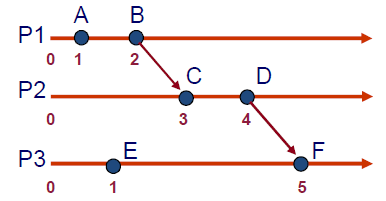
\includegraphics[scale=0.5]{src/images/synchronization/scalar-clock.png}
    \centering
\end{figure}

\textbf{Note that}, this procedure give us only a partial order. In order to achieve a total order we can simply attach the process ID to the integer counter, so, for example, counter $1.3$ tells us that the current counter value is $1$ in process $3$. It's important to notice that achieve a total order doesn't mean there are no parallel events.

\subsubsection{Vector clocks}
In scalar clocks, from the \textit{happens-before} relationship we know that $e \rightarrow e' \implies L(e) < L(e')$ but, as we can see, this is an implication, not a double implication, so the reverse doesn't necessary hold. In order to solve this problem there were introduced the vector clocks.

\paragraph{Implementation}

In vector clocks each process maintains a vector of $N$ values (where $N$ is the number of processes), such that every process has a snapshot of the situation of the other processes.\\
So, let's define the vector $V_i[N]$ as the vector of the process $i$. Each process $i$ knows something about the situation of other processes, so if we have $V_i[j] = k$, this means that process $i$ knows that $k$ events occurred in process $j$.

\begin{itemize}
    \item \textit{Initial condition}: every process has a vector where all cells are initialized at 0, so $V_i[j] = 0 \forall i, j$
    \item Every time a message is sent by process $i$, this is timestamped with $L_i$
    \item Increments:
    \begin{enumerate}
        \item $V_i[i]$ is incremented just before process $i$ sends a message
        \item Upon receipt of a message, process $i$ sets $V_i[j] = \texttt{MAX}(ts(msg), V_i[j]) \texttt{  } \forall i \neq j$, where $ts(msg)$ is the timestamp contained in the message received, and then increments $V_i[i]$.
    \end{enumerate}
\end{itemize}

\begin{figure}[h]
    \caption{An example of vector clock implementation}
    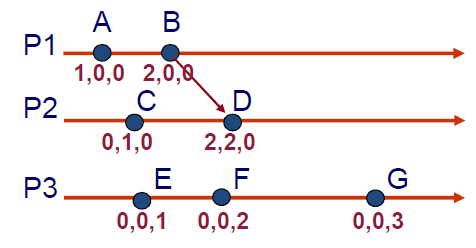
\includegraphics[scale=0.5]{src/images/synchronization/vector-clock.png}
    \centering
\end{figure}

\paragraph{Causal delivery}
We can also use vector clocks, with slight variations, in order to implement causal delivery of messages in a totally distributed way. In practice, we increment the clock only when sending a message and, on receive, we just merge, without any increment.

\begin{figure}[h]
    \caption{An example of vector clock implementation}
    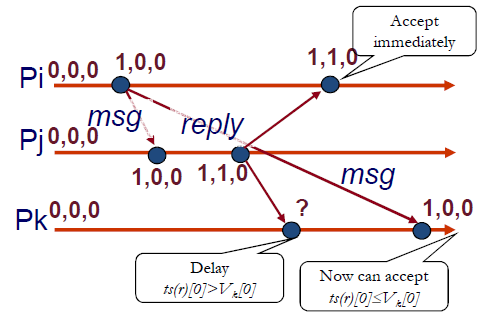
\includegraphics[scale=0.5]{src/images/synchronization/vector-clock-causality.png}
    \centering
\end{figure}

\subsection{Mutual exclusion}
The \textbf{mutual exclusion} aims to prevent interference and ensure consistency of resource access among several processes. In order to face up with this problem we assume to have \textbf{reliable channels and processes}. Moreover, the mutual exclusion has to satisfy two main requirements: \textbf{safety}, which means than only one process may execute in the critical section at a time, and \textbf{liveness}, which means that all requests to enter/exit the critial section eventually succeed.

\subsubsection{Mutual exclusion with scalar clocks}
The procedure is pretty simple and it exploits the scalar clock methodology with the goal to use timestamps as a metric for resource assignment.

In details, a process multicasts a resource request message to all processes, including its timestamp. When processes receive the message, they have three options:
\begin{enumerate}
    \item If it doesn't hold the resource and it's not interested to hold it, simply replies with an \textit{ACK}
    \item If it holds the resource, puts the requests into a local queue ordered according to timestamps
    \item If it doesn't hold the resource, it's interested to hold it but it has already sent a request message, it replies with an \textit{ACK} if the incoming request message has a lower timestamp, otherwise put it on a local queue
\end{enumerate}
When releasing a resource, a process acknowledges all the requests queued and the resource is granted to a process when its request has been acknowledged by all processes.

\subsubsection{Token ring solution}
